\documentclass{article}          
\usepackage{tikz}
\usetikzlibrary{arrows}

\definecolor{myblue}{RGB}{56,94,141}
\begin{document}

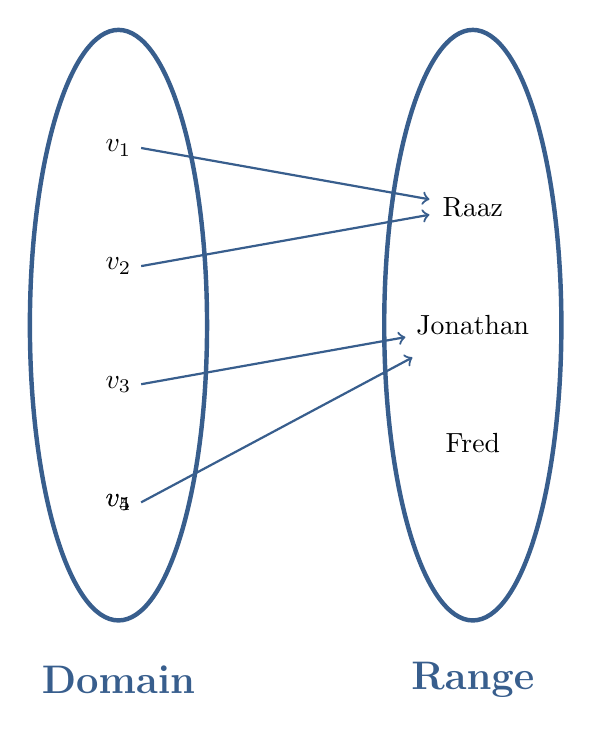
\begin{tikzpicture}[scale=.75]
\draw[ultra thick,myblue] (0,0) circle [x radius=1.5cm, y radius=5cm]
                    (6,0) circle [x radius=1.5cm, y radius=5cm];
\node[font=\color{myblue}\Large\bfseries] at (0,-6) {Domain};
\node[font=\color{myblue}\Large\bfseries] at (6,-6) {Range};  

\node (a1) at (0,3)  {$v_{1}$};
\node (a2) at (0,1)   {$v_2$};
\node (a3) at (0,-1)  {$v_3$};
\node (a4) at (0,-3)  {$v_4$};
\node (a4) at (0,-3)  {$v_5$};


\node[circle] (b1) at (6,2)  {Raaz}; 
 % I used circle to get a fine position of the arrows without a complicated code
\node[circle] (b2) at (6,0)  {Jonathan};
\node[circle] (b3) at (6,-2) {Fred};

\draw[thick,->,myblue] (a1.east) -- (b1);
\draw[thick,->,myblue] (a2.east) -- (b1);
\draw[thick,->,myblue] (a3.east) -- (b2);
\draw[thick,->,myblue] (a4.east) -- (b2);
\end{tikzpicture}    
\end{document} 
